
% This must be in the first 5 lines to tell arXiv to use pdfLaTeX, which is strongly recommended.
\pdfoutput=1
% In particular, the hyperref package requires pdfLaTeX in order to break URLs across lines.

\documentclass[11pt]{article}

% Change "review" to "final" to generate the final (sometimes called camera-ready) version.
% Change to "preprint" to generate a non-anonymous version with page numbers.
\usepackage[review]{acl}

% Standard package includes
\usepackage{times}
\usepackage{latexsym}

% For proper rendering and hyphenation of words containing Latin characters (including in bib files)
\usepackage[T1]{fontenc}
% For Vietnamese characters
% \usepackage[T5]{fontenc}
% See https://www.latex-project.org/help/documentation/encguide.pdf for other character sets

% This assumes your files are encoded as UTF8
\usepackage[utf8]{inputenc}

% This is not strictly necessary, and may be commented out,
% but it will improve the layout of the manuscript,
% and will typically save some space.
\usepackage{microtype}

% This is also not strictly necessary, and may be commented out.
% However, it will improve the aesthetics of text in
% the typewriter font.
\usepackage{inconsolata}

%Including images in your LaTeX document requires adding
%additional package(s)
\usepackage{graphicx}
\usepackage{setspace}
\usepackage{graphicx}
\usepackage{listings}
\usepackage{xcolor}
\usepackage{subcaption}
\usepackage{import}

% Add this line to define \textrussian command
\newcommand{\textrussian}[1]{\foreignlanguage{russian}{#1}}

\lstset{
    language=Python,
    breaklines=true,
    basicstyle=\ttfamily,
    keywordstyle=\color{blue},
    linewidth=0.5\textwidth,  % Set the width to 90% of the text width
}
\usepackage{graphicx}
\graphicspath{{/Users/HansPeter/Dev/ku_local/NLP-course/src/nlp_course/plots}}


\begin{document}


\title{NLP Course Report}
\author{Hans Peter Lyngsøe, pvr448}

\maketitle

\section{Week 1}
% (a) Explore the dataset from https://huggingface.co/datasets/coastalcph/tydi_xor_rc. 
% Familiarize yourself with the dataset card, download the dataset and explore its columns. 
% Summarize basic data statistics for training and validation data in each of the languages 
% Finnish (fi), Japanese (ja) and Russian (ru).
\begin{enumerate}
    \item[(a)] 

    Basic statistics:
    \begin{itemize}
        \item the data is quite evenly distributed across the 3 languages.
        \item We note that there are more answerable than unanswerable by a factor of 10-1.
        \item train\_set: 15326
        \item val\_set: 3028
    \end{itemize}

    \begin{figure}[ht]
        \centering
        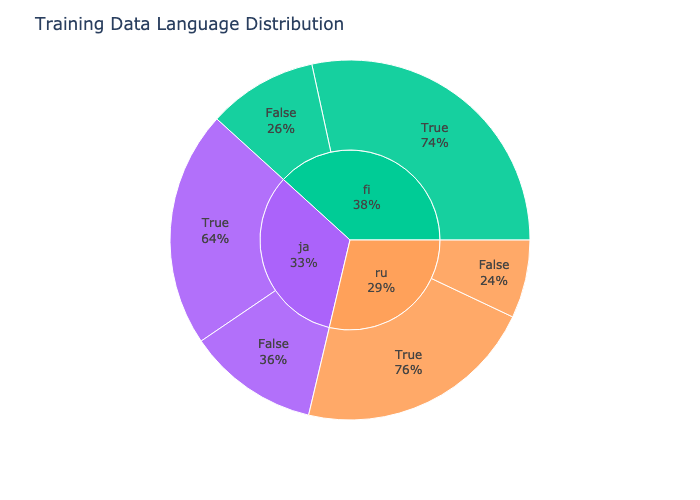
\includegraphics[width=0.5\textwidth]{week1_a_dataset.png}
        \caption{Distribution of labels in the dataset}
        \label{fig:label_distribution}
    \end{figure}

    \begin{figure}[ht]
        \centering
        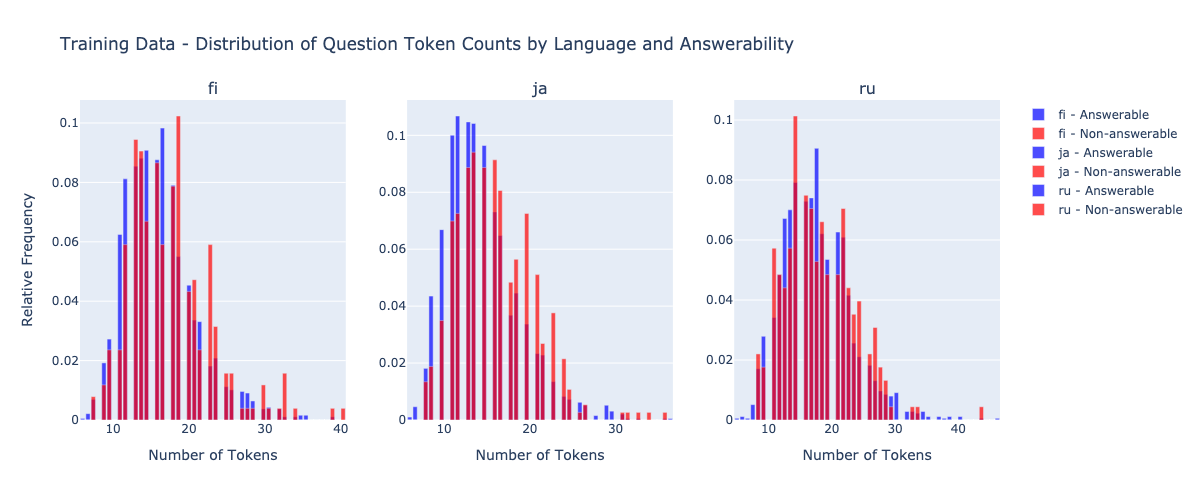
\includegraphics[width=0.5\textwidth]{week1_a_lang_token_distribution_normalized.png}
        \caption{normalized Histogram for token count(using llama3 tokenizer) of answerable/unanswerable questions in the dataset}
        \label{fig:language_distribution}
    \end{figure}

    % (b) For each of the languages Finnish, Japanese and Russian, report the 5 most common 
    % words in the questions from the training set. What kind of words are they?
    \item[(b)] 

    In order to get a faithful representation of the most meaningful words, we opt to filter out stopwords arguing that these words are not meaningful and does not carry information about the question.
    We use the NLP library spacy that provides and index of stopwords for each language.

    we use the fact that both finnish and russian uses spaces to seperate their words, and thus we can extract distinct words using the space as delimiter.

    Japanese is somewhat different as a language, and it is unclear whether naive splitting on space is meaningfull. 
    Thus we use a japanese speific tokenizer to parse sentences into words.

    \begin{lstlisting}[language=Python]
    import MeCab
    def get_top_words(df: pd.DataFrame, lang: str, n=5):
        df_lang = df[df['lang'] == lang].copy()
        
        if lang == 'ja':
            mecab = MeCab.Tagger("-Owakati")  # Initialize MeCab tokenizer
            df_lang.loc[:, 'words_question_tokens'] = df_lang['question'].apply(lambda x: mecab.parse(x).split())
        else:
            df_lang.loc[:, 'words_question_tokens'] = df_lang['question'].apply(lambda x: x.split(' '))
        
        all_tokens = np.concatenate(df_lang['words_question_tokens'].values)
        unique, counts = np.unique(all_tokens, return_counts=True)
        sorted_indices = np.argsort(counts)[::-1]
        top_unique_tokens = unique[sorted_indices][:n]
        top_tokens_dict = {token: int(count) for token, count in zip(top_unique_tokens, counts[sorted_indices][:n])}
        return top_tokens_dict
    \end{lstlisting}


    we get the following results:

    \begin{figure}[t]
        \centering
        \begin{subfigure}[b]{0.1\textwidth}
            \centering
            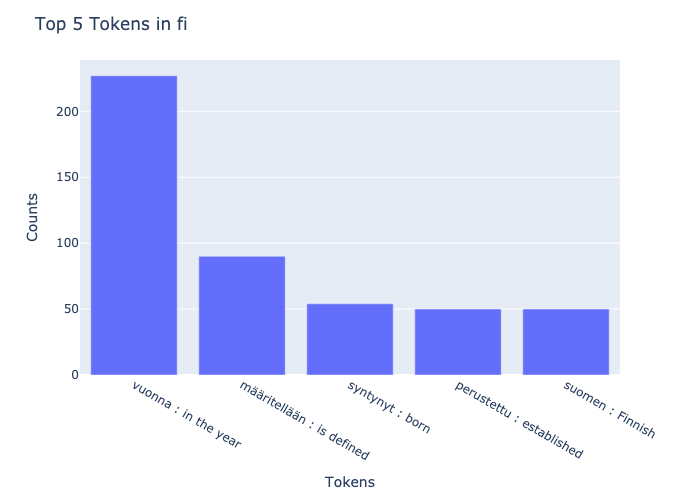
\includegraphics[width=\textwidth]{week1_b_top_5_tokens_fi.png}
            \caption{Finnish}
            \label{fig:top_5_tokens_fi}
        \end{subfigure}
        \hfill
        \begin{subfigure}[b]{0.1\textwidth}
            \centering
            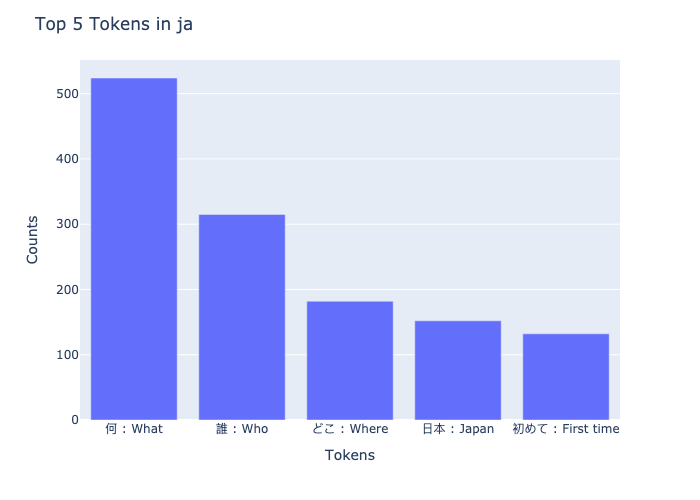
\includegraphics[width=\textwidth]{week1_b_top_5_tokens_ja.png}
            \caption{Japanese}
            \label{fig:top_5_tokens_ja}
        \end{subfigure}
        \hfill
        \begin{subfigure}[b]{0.1\textwidth}
            \centering
            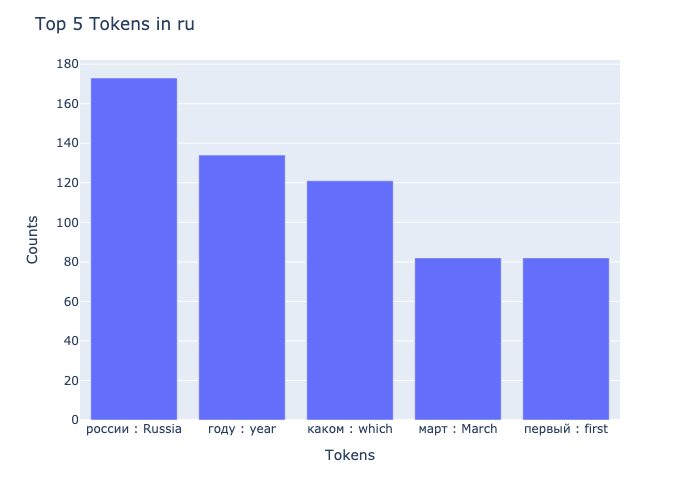
\includegraphics[width=\textwidth]{week1_b_top_5_tokens_ru.png}
            \caption{Russian}
            \label{fig:top_5_tokens_ru}
        \end{subfigure}
        \caption{Top 5 tokens in Finnish, Japanese, and Russian}
        \label{fig:top_5_tokens_all}
    \end{figure}

    NOTE: todo use an embedding model to get a sense for the meaning of the words, consider how you do tokenization and 
    what the implications are. what are words and what are stopwords

% (c) Implement a rule-based classifier that predicts whether a question is answerable 
% or impossible, only using the document (context) and question. You may use machine 
% translation as a component. Use the answerable field to evaluate it on the validation set. 
% What is the performance of your classifier for each of the languages Finnish, Japanese and Russian?
    \item[(c)] 
    
    As a simple rule based approach explore the relationship between word/token count and answerability in the training set. 

    We expect that there is a rough heuristic that question are harder to answer for longer questions. 

    \begin{figure}[ht]
        \centering
        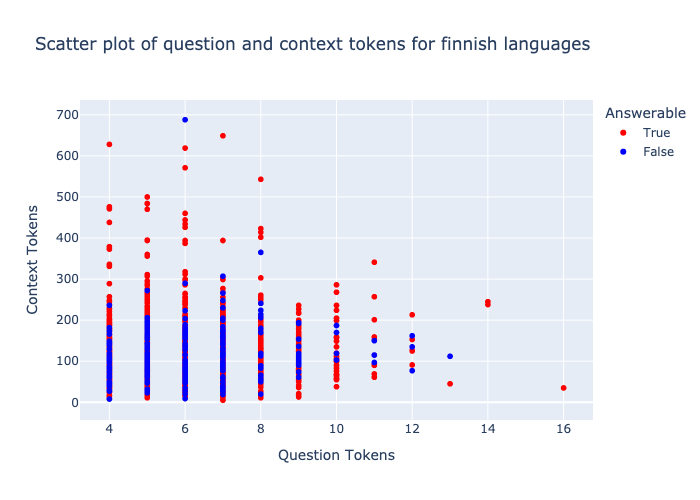
\includegraphics[width=0.5\textwidth]{week1_c_scatter_fi.png}
        \caption{Scatter plot for Finnish}
        \label{fig:scatter_fi}
    \end{figure}

    \begin{figure}[ht]
        \centering
        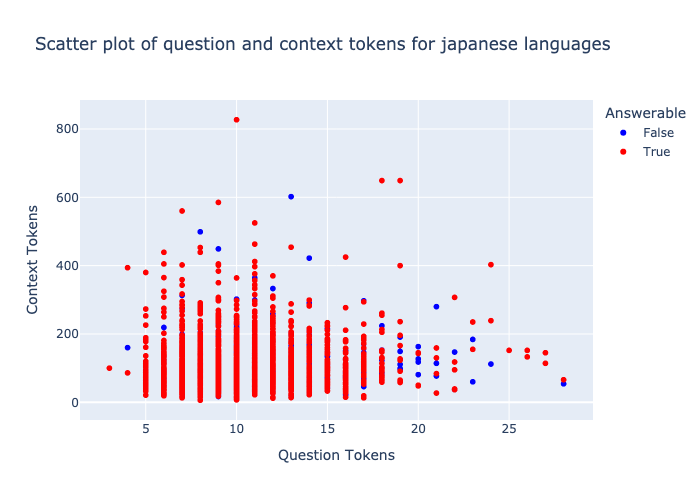
\includegraphics[width=0.5\textwidth]{week1_c_scatter_ja.png}
        \caption{Scatter plot for Japanese}
        \label{fig:scatter_ja}
    \end{figure}
    
    \begin{figure}[ht]
        \centering
        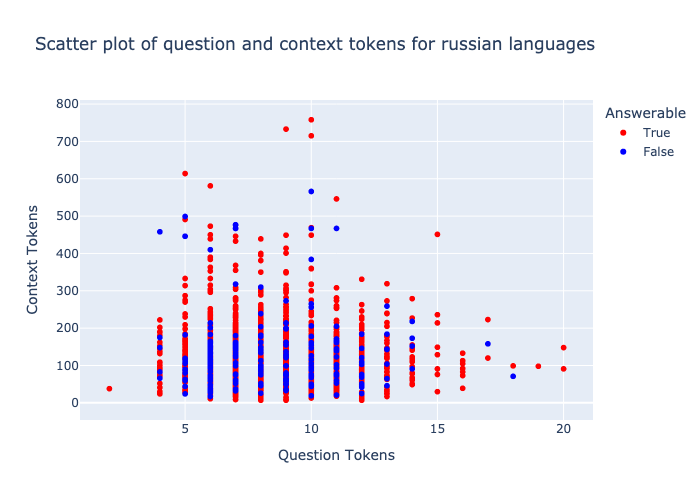
\includegraphics[width=0.5\textwidth]{week1_c_scatter_ru.png}
        \caption{Scatter plot for Russian}
        \label{fig:scatter_ru}
    \end{figure}


    based on this information, we decide to make a rule based classifier that predicts unanwerable for questions containing less than 15 words/subwords.

    we get the following results on the validation set:

    %% 0.6210144927536232, 'f1': 0.7263212977498692, 'precision': 0.7486515641855448, 'recall': 0.7052845528455285
    %%  japanese {'accuracy': 0.6140350877192983, 'f1': 0.7411764705882353, 'precision': 0.6511627906976745, 'recall': 0.8600682593856656}
    %% russian 'accuracy': 0.75, 'f1': 0.8571428571428571, 'precision': 0.7538071065989848, 'recall': 0.9933110367892977
    \begin{table}[ht]
        \centering
        \begin{tabular}{|l|c|c|c|c|}
            \hline
            Language & Accuracy & F1 Score & Precision & Recall \\
            \hline
            All & 0.62 & 0.726 & 0.749 & 0.705 \\
            Finnish (fi) & 0.7424 & 0.8522 & 0.7424 & 1.0000 \\
            Japanese (ja) & 0.6140 & 0.7412 & 0.6512 & 0.8601 \\
            Russian (ru) & 0.7500 & 0.8571 & 0.7538 & 0.9933 \\
            \hline
        \end{tabular}
        \caption{Performance metrics of the rule-based classifier on the validation set}
        \label{tab:classifier_performance}
    \end{table}

    downsides:
        we have one rule for all languages. relies heavily on tokenization and assuming that languages have similar structures.
        this model is putting a lot of faith in the tokenization step.

\end{enumerate}

\section{Week 37 (9--15 September)}
% Let k be the number of members in your group (k ∈ {1, 2, 3}). Implement k different 
% language models for the questions in the three languages Finnish, Japanese and Russian, 
% as well as for the document contexts in English (total k × 4 language models), using the 
% training data. Evaluate each of them on the validation data, report their performance 
% and discuss the results.


\begin{table}[ht]
    \centering
    \begin{tabular}{|l|r|r|}
        \hline
        Language & Training Tokens/Words & Perplexity \\
        \hline
        Japanese (ja) & 24,533 & 548.79 \\
        Russian (ru) & 16,526 & 140.53 \\
        Finnish (fi) & 13,013 & 91.90 \\
        Context (English) & 751,154 & 616.85 \\
        \hline
    \end{tabular}
    \caption{Language Model Performance}
    \label{tab:language_model_performance}
\end{table}



\section{Week 38 (16--22 September)}
% Let k be the number of members in your group. For each of the three languages Finnish, 
% Japanese and Russian separately, using the training data, train k different classifiers 
% that receive the document (context) and question as input and predict whether the question 
% is answerable or impossible given the context. Evaluate the classifiers on the respective 
% validation sets, report and analyse the performance for each language and compare the 
% scores across languages.

We opt for a simple linear model on top of openai embedding matryoshka embedding model. 
We embed the question and context and concatenate them into one feature vector. 
This gives us a feature space of dimension 3072.

We argue that a combination of the embedding context and question would lead to improved results 

\begin{table}[ht]
    \centering
    \resizebox{\textwidth}{!}{%
    \begin{tabular}{|l|l|c|c|c|c|c|c|}
    \hline
    Training & Evaluation & Context & D\_in & Expansion & Balanced & Precision & Recall \\
    & & & & Factor & Accuracy & & \\
    \hline
    Finnish & Finnish & No & 1536 & 2 & 0.7045 & 0.9664 & 1.0000 \\
    Finnish & Finnish & Yes & 3072 & 2 & 0.7955 & 0.9765 & 1.0000 \\
    Japanese & Japanese & No & 1536 & 2 & 0.7625 & 0.9105 & 0.9519 \\
    Japanese & Japanese & Yes & 3072 & 2 & 0.5244 & 0.8274 & 1.0000 \\
    Russian & Russian & No & 1536 & 2 & 0.9031 & 0.9825 & 0.9492 \\
    Russian & Russian & Yes & 3072 & 2 & 0.7058 & 0.9355 & 0.9831 \\
    \hline
    \end{tabular}%
    }
    \caption{Model performance for language-specific and combined training, with and without context}
    \label{tab:model_performance}
\end{table}

we also try to train a single model for all languages which meaningfully boosts performance 
but when context embedding is included and when it is n

\begin{table}[ht]
    \centering
    \resizebox{\textwidth}{!}{%
    \begin{tabular}{|l|l|c|c|c|c|c|c|}
    \hline
    Training & Evaluation & Context & D\_in & Expansion & Balanced & Precision & Recall \\
    & & & & Factor & Accuracy & & \\
    \hline
    All & Finnish & No & 1536 & 2 & 0.9414 & 0.9933 & 0.9364 \\
    All & Finnish & Yes & 3072 & 2 & 0.9225 & 0.9888 & 0.9343 \\
    All & Japanese & No & 1536 & 2 & 0.6688 & 0.8741 & 0.9840 \\
    All & Japanese & Yes & 3072 & 2 & 0.8663 & 0.9559 & 0.9278 \\
    All & Russian & No & 1536 & 2 & 0.7955 & 0.9765 & 1.0000 \\
    All & Russian & Yes & 3072 & 2 & 0.8810 & 0.9867 & 0.9893 \\
    \hline
    \end{tabular}%
    }
    \caption{Model performance for language-specific and combined training, with and without context}
    \label{tab:model_performance}

\end{table}






\section{Week 39 (23--29 September)}
% We now move from binary classification to span-based QA, i.e. identifying the
% span in the document that answers the question.
% Let k be the number of members in your group. Using the training data in
% Finnish, Japanese and Russian separately, train k different sequence labellers,
% which predict the tokens in a document context that constitute the answer to
% the corresponding question.9 You can decide whether to train one model per
% language or a single model for all three languages. Evaluate using a sequence la-
% belling metric on the validation set, report and analyse the performance for each
% language and compare the scores across languages. Note that if the question is
% unanswerable, a correct output must be empty (contain no tokens).


\section{Week 40 (30 September--6 October)}
% Use the subset of the questions in Finnish, Japanese and Russian to train (or fine-tune) 
% an encoder-decoder model that receives the question and context as input and generates 
% the in-language answer. You can decide whether to train one model per language or a 
% single model for all three languages.

\section{Week 41+ (from 7 October)}
% Use all questions in Finnish, Japanese and Russian to train (or fine-tune) an encoder-decoder 
% model that receives the question and context as input and generates the English answer. 
% You can decide whether to train one model per question language or a single model for all 
% three languages. Evaluate using a text generation metric on the validation set, and compare 
% the overall results between answerable and unanswerable examples.


\section{Document Body}

\subsection{Footnotes}

Footnotes are inserted with the \verb|\footnote| command.\footnote{This is a footnote.}

\subsection{Tables and figures}

See Table~\ref{tab:accents} for an example of a table and its caption.
\textbf{Do not override the default caption sizes.}

\begin{table}
  \centering
  \begin{tabular}{lc}
    \hline
    \textbf{Command} & \textbf{Output} \\
    \hline
    \verb|{\"a}|     & {\"a}           \\
    \verb|{\^e}|     & {\^e}           \\
    \verb|{\`i}|     & {\`i}           \\
    \verb|{\.I}|     & {\.I}           \\
    \verb|{\o}|      & {\o}            \\
    \verb|{\'u}|     & {\'u}           \\
    \verb|{\aa}|     & {\aa}           \\\hline
  \end{tabular}
  \begin{tabular}{lc}
    \hline
    \textbf{Command} & \textbf{Output} \\
    \hline
    \verb|{\c c}|    & {\c c}          \\
    \verb|{\u g}|    & {\u g}          \\
    \verb|{\l}|      & {\l}            \\
    \verb|{\~n}|     & {\~n}           \\
    \verb|{\H o}|    & {\H o}          \\
    \verb|{\v r}|    & {\v r}          \\
    \verb|{\ss}|     & {\ss}           \\
    \hline
  \end{tabular}
  \caption{Example commands for accented characters, to be used in, \emph{e.g.}, Bib\TeX{} entries.}
  \label{tab:accents}
\end{table}

As much as possible, fonts in figures should conform
to the document fonts. See Figure~\ref{fig:experiments} for an example of a figure and its caption.

Using the \verb|graphicx| package graphics files can be included within figure
environment at an appropriate point within the text.
The \verb|graphicx| package supports various optional arguments to control the
appearance of the figure.
You must include it explicitly in the \LaTeX{} preamble (after the
\verb|\documentclass| declaration and before \verb|\begin{document}|) using
\verb|\usepackage{graphicx}|.

\begin{figure}[t]
  \includegraphics[width=\columnwidth]{example-image-golden}
  \caption{A figure with a caption that runs for more than one line.
    Example image is usually available through the \texttt{mwe} package
    without even mentioning it in the preamble.}
  \label{fig:experiments}
\end{figure}

\begin{figure*}[t]
  \includegraphics[width=0.48\linewidth]{example-image-a} \hfill
  \includegraphics[width=0.48\linewidth]{example-image-b}
  \caption {A minimal working example to demonstrate how to place
    two images side-by-side.}
\end{figure*}

\subsection{Hyperlinks}

Users of older versions of \LaTeX{} may encounter the following error during compilation:
\begin{quote}
\verb|\pdfendlink| ended up in different nesting level than \verb|\pdfstartlink|.
\end{quote}
This happens when pdf\LaTeX{} is used and a citation splits across a page boundary. The best way to fix this is to upgrade \LaTeX{} to 2018-12-01 or later.

\subsection{Citations}

\begin{table*}
  \centering
  \begin{tabular}{lll}
    \hline
    \textbf{Output}           & \textbf{natbib command} & \textbf{ACL only command} \\
    \hline
    \citep{Gusfield:97}       & \verb|\citep|           &                           \\
    \citealp{Gusfield:97}     & \verb|\citealp|         &                           \\
    \citet{Gusfield:97}       & \verb|\citet|           &                           \\
    \citeyearpar{Gusfield:97} & \verb|\citeyearpar|     &                           \\
    \citeposs{Gusfield:97}    &                         & \verb|\citeposs|          \\
    \hline
  \end{tabular}
  \caption{\label{citation-guide}
    Citation commands supported by the style file.
    The style is based on the natbib package and supports all natbib citation commands.
    It also supports commands defined in previous ACL style files for compatibility.
  }
\end{table*}

Table~\ref{citation-guide} shows the syntax supported by the style files.
We encourage you to use the natbib styles.
You can use the command \verb|\citet| (cite in text) to get ``author (year)'' citations, like this citation to a paper by \citet{Gusfield:97}.
You can use the command \verb|\citep| (cite in parentheses) to get ``(author, year)'' citations \citep{Gusfield:97}.
You can use the command \verb|\citealp| (alternative cite without parentheses) to get ``author, year'' citations, which is useful for using citations within parentheses (e.g. \citealp{Gusfield:97}).

A possessive citation can be made with the command \verb|\citeposs|.
This is not a standard natbib command, so it is generally not compatible
with other style files.

\subsection{References}

\nocite{Ando2005,andrew2007scalable,rasooli-tetrault-2015}

The \LaTeX{} and Bib\TeX{} style files provided roughly follow the American Psychological Association format.
If your own bib file is named \texttt{custom.bib}, then placing the following before any appendices in your \LaTeX{} file will generate the references section for you:
\begin{quote}
\begin{verbatim}
\bibliography{custom}
\end{verbatim}
\end{quote}

You can obtain the complete ACL Anthology as a Bib\TeX{} file from \url{https://aclweb.org/anthology/anthology.bib.gz}.
To include both the Anthology and your own .bib file, use the following instead of the above.
\begin{quote}
\begin{verbatim}
\bibliography{anthology,custom}
\end{verbatim}
\end{quote}

Please see Section~\ref{sec:bibtex} for information on preparing Bib\TeX{} files.

\subsection{Equations}

An example equation is shown below:
\begin{equation}
  \label{eq:example}
  A = \pi r^2
\end{equation}

Labels for equation numbers, sections, subsections, figures and tables
are all defined with the \verb|\label{label}| command and cross references
to them are made with the \verb|\ref{label}| command.

This an example cross-reference to Equation~\ref{eq:example}.

\subsection{Appendices}

Use \verb|\appendix| before any appendix section to switch the section numbering over to letters. See Appendix~\ref{sec:appendix} for an example.

\section{Bib\TeX{} Files}
\label{sec:bibtex}


\end{document}